\begin{enumerate}
	\item \textbf{Activate Voter}
		\begin{enumerate}
			\item \textbf{Service Contract}
				\begin{figure}[H]
					\centering
					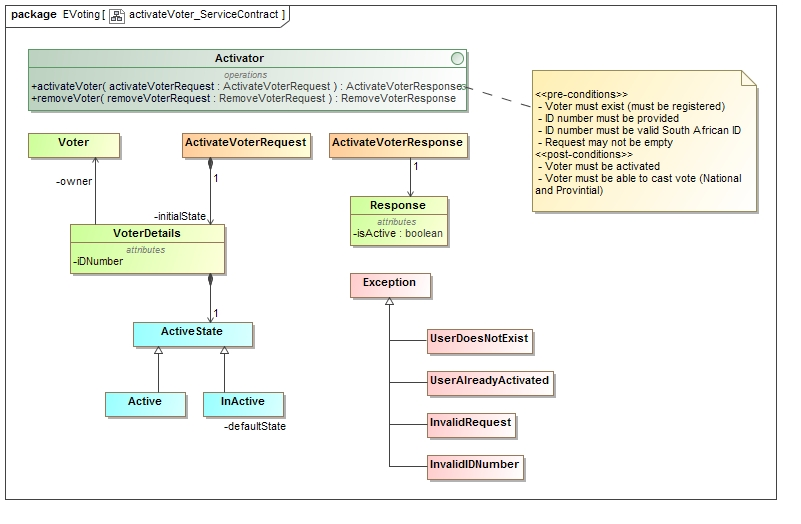
\includegraphics[width=0.75\linewidth]{../Images/Activator/ServiceContract/activateVoter_ServiceContract.jpg}
					\caption{Activate Voter Service Contract}
				\end{figure}
				
				Activate Voter requires an ID number in the request which will be used to change the ActiveState state to active if all pre-conditions are met.
				\newline				
				
				\begin{enumerate}
					\item Pre-conditions
					\begin{itemize}
						\item An ID number must be present in the request.
						\item The ID number must be a valid South African ID number.
						\item Voter must exist (must be a registered voter).
						\item The voter must not already be registered.
					\end{itemize}
					
					\item Exceptions
					\begin{itemize}
						\item If the ID number is not a valid South African ID, the invalidIDNumber exception will be thrown.
						\item If the user does not exist in the database, the userDoesNotExist exception will be thrown.
						\item If the user is already activated, the userAlreadyActivated exception will be thrown.
					\end{itemize}
					
					\item Post-conditions
					\begin{itemize}
						\item The Voter's ActivateState must be Active.
					\end{itemize}
				\end{enumerate}
			
			\newpage
			
			\item \textbf{Functional Requirements}
				\begin{figure}[H]
					\centering
					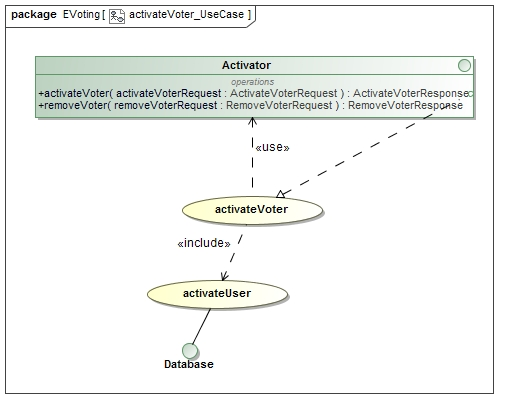
\includegraphics[width=0.75\linewidth]{../Images/Activator/UseCase/activateVoter_UseCase.jpg}
					\caption{Activate User Use Case}
				\end{figure}
				
				The Activate Voter process will call the ActivateUser use case from the database module.
				\newline
			\newpage
			\item \textbf{Process Design}
				\begin{figure}[H]
					\centering
					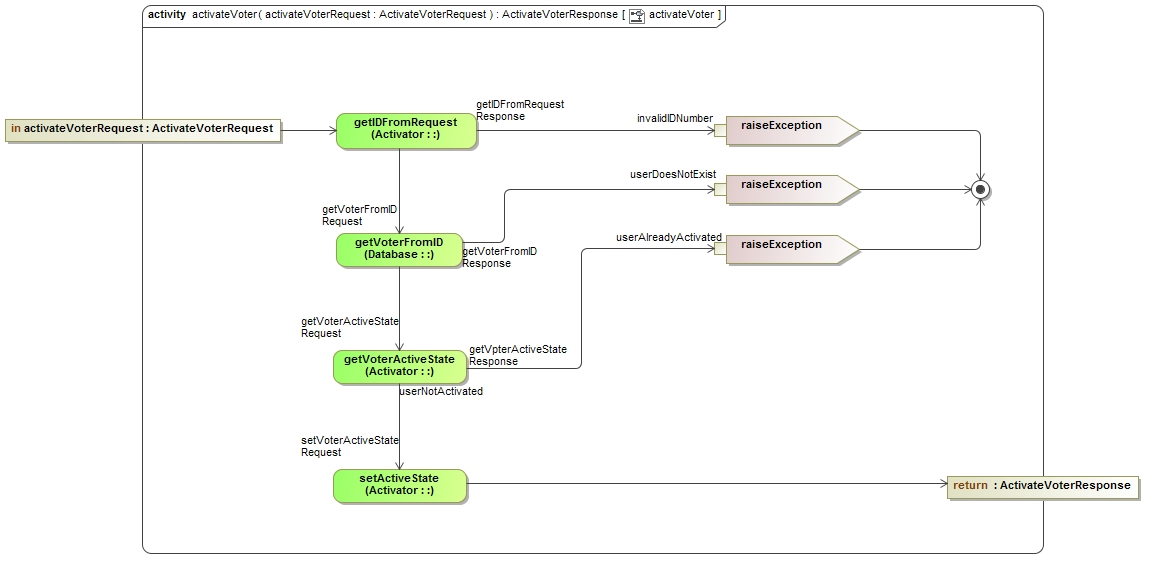
\includegraphics[width=0.75\linewidth]{../Images/Activator/Activity/activateVoter.jpg}
					\caption{Activate User Activity}
				\end{figure}
				
				The Activate Voter process will first retrieve the ID number from the request and validate if is a valid ID number, after which it will get all the necessary Voter details from the database wich corresponds to that ID number. It then checks in what state the voter is to see if it has already been activated. If all cases are valid, then the voter's ActiveState will change from Invalid to Valid.
				\newline
		\end{enumerate}
	
	\item \textbf{Remove Voter}
		\begin{enumerate}
			\item \textbf{Service Contract}
			\begin{figure}[H]
				\centering
				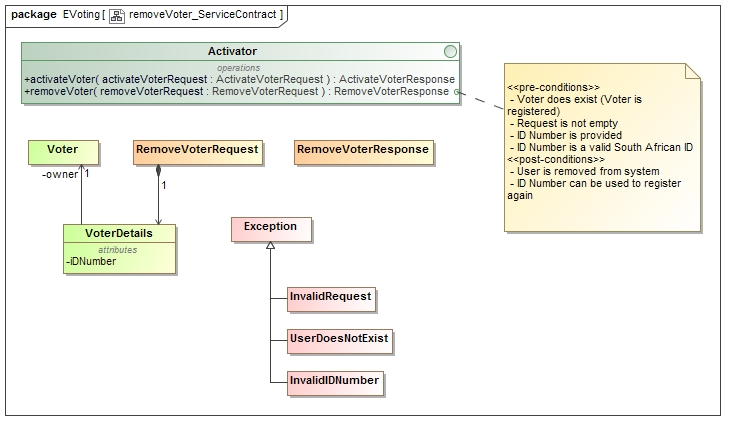
\includegraphics[width=0.75\linewidth]{../Images/Activator/ServiceContract/removeVoter_ServiceContract.jpg}
				\caption{Remove Voter Service Contract}
			\end{figure}
			
			There are cases where the Activator will need to be able to remove a user. In the removeActivatorRequest, an ID number must be provided so that the voter associated with that ID number be removed from the system.
			\newline
			
			\begin{enumerate}
				\item Pre-conditions
				\begin{itemize}
					\item An ID number must be provided.
					\item The ID number must be a valid South African ID.
					\item The user must exist in the system.
				\end{itemize}
				
				\item Exceptions
				\begin{itemize}
						\item If the ID number in the request is not a valid ID number, the InvalidIDNumber exception will be thrown.
						\item If the user does not exist in the database, the userDoesNotExist exception will be thrown.
				\end{itemize}
				
				\item Post-conditions
				\begin{itemize}
					\item The user is removed from the system.
				\end{itemize}
			\end{enumerate}
			
			\item \textbf{Functional Requirements}
			\begin{figure}[H]
				\centering
				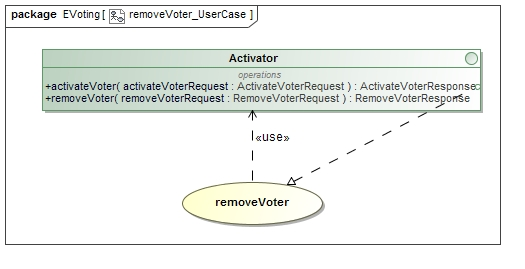
\includegraphics[width=0.75\linewidth]{../Images/Activator/UseCase/removeVoter_UserCase.jpg}
				\caption{Remove Voter Use Case}
			\end{figure}
			
			The removeVoter will call a method of the database to remove the voter with that ID number. The database module is not fully documented as of yet.
			\newline
			\newpage
			\item \textbf{Process Design}
			\begin{figure}[H]
				\centering
				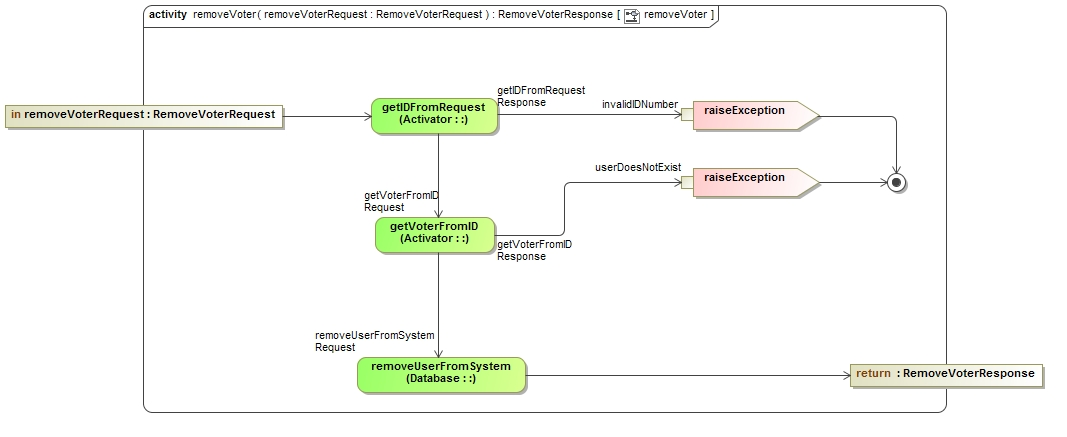
\includegraphics[width=0.75\linewidth]{../Images/Activator/Activity/removeVoter.jpg}
				\caption{Remove Voter Activity}
			\end{figure}
			
				The Remove Voter process will first retrieve the ID number from the request and validate if is a valid ID number. If a user associated with that ID number is found, the process will call a function from the database module to remove the user from the system.
			\newline
		\end{enumerate}
\end{enumerate}